\documentclass{article}
\usepackage{tikz,pgfplots}
\begin{document}
    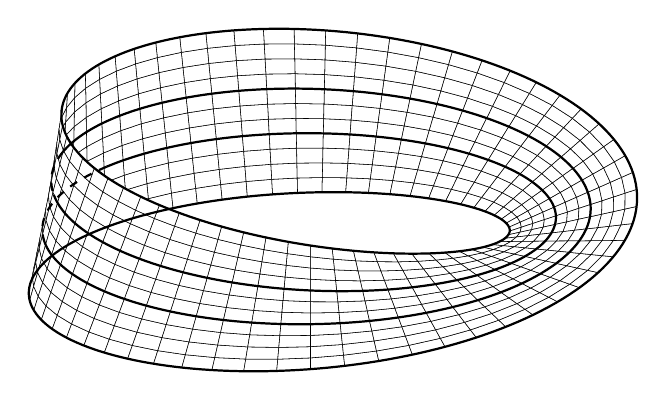
\begin{tikzpicture}
        \begin{axis}[width=12cm,height=8cm,hide axis,view={30}{50}]
            \addplot3[surf,very thin,faceted color=black,colormap={white}{color(0cm)=(white); color(1cm)=(white)},samples=60,samples y=12,domain=0:360,y domain=-0.5:0.5,z buffer=sort]
            ({(1+0.5*y*cos(x/2))*cos(x)},{(1+0.5*y*cos(x/2))*sin(x)},{0.5*y*sin(x/2)});
            \addplot3[thick,black,domain=0:360,samples=200,samples y=0]
            ({(1+0.25*cos(x/2))*cos(x)},{(1+0.25*cos(x/2))*sin(x)},{0.25*sin(x/2)});
            \addplot3[thick,black,domain=0:190,samples=200,samples y=0]
            ({(1+0.06818*cos(x/2))*cos(x)},{(1+0.06818*cos(x/2))*sin(x)},{0.06818*sin(x/2)});
            \addplot3[dashed,thick,black,domain=190:215,samples=200,samples y=0]
            ({(1+0.06818*cos(x/2))*cos(x)},{(1+0.06818*cos(x/2))*sin(x)},{0.06818*sin(x/2)});
            \addplot3[thick,black,domain=215:360,samples=200,samples y=0]
            ({(1+0.06818*cos(x/2))*cos(x)},{(1+0.06818*cos(x/2))*sin(x)},{0.06818*sin(x/2)});
            \addplot3[thick,black,domain=0:360,samples=200,samples y=0]
            ({(1-0.25*cos(x/2))*cos(x)},{(1-0.25*cos(x/2))*sin(x)},
            {-0.25*sin(x/2)});
            \addplot3[thick,black,domain=0:170,samples=200,samples y=0]
            ({(1-0.06818*cos(x/2))*cos(x)},{(1-0.06818*cos(x/2))*sin(x)},{-0.06818*sin(x/2)});
            \addplot3[dashed,thick,black,domain=170:215,samples=200,samples y=0]
            ({(1-0.06818*cos(x/2))*cos(x)},{(1-0.06818*cos(x/2))*sin(x)},{-0.06818*sin(x/2)});
            \addplot3[thick,black,domain=215:360,samples=200,samples y=0]
            ({(1-0.06818*cos(x/2))*cos(x)},{(1-0.06818*cos(x/2))*sin(x)},{-0.06818*sin(x/2)});
        \end{axis}
    \end{tikzpicture}
\end{document}